\chapter{Multiplication I: schoolbook, Karatsuba, and Toom}
\label{ch:mul}

Multiplication is the operation that matters most. Division, square roots, decimal
conversion, and powers are all built out of multiplications, so their speed follows
multiplication's speed. The default dispatcher starts with schoolbook, then uses
Karatsuba (which can split three ways), then switches to the NTT.

\begin{center}
\begin{tikzpicture}
  \foreach \x/\c/\t/\s in {0/sAqua/schoolbook/{$n^2$},1/sBlue/Karatsuba/{$n^{1.585}$},2/sViolet/Toom-3/{$n^{1.465}$},3/sOrange/NTT/{$n\log n$}} {
    \node[algo,fill=\c,minimum width=27mm] at (\x*3,0) {\t\\[-1pt]\footnotesize\s};
  }
  \draw[arr] (-1.3,-0.75) -- node[below,lbl]{larger operands $\rightarrow$ methods with more setup and less growth} (10.3,-0.75);
\end{tikzpicture}
\end{center}

This chapter explains the direct multiplication methods, including the
experimental higher-degree Toom splits. \Cref{ch:ntt,ch:fermat} cover transform methods.
\Cref{ch:muldispatch} explains how the library chooses.

\section{Schoolbook multiplication}
\label{sec:schoolbook}

This is long multiplication as taught in school: multiply the first number by each limb
of the second, shift each partial product one limb further left, and add them all up.

\begin{example}[: $123 \times 45$ in base 10]
\[
\begin{array}{c@{\,}c@{\,}c@{\,}c@{\,}c@{\qquad}l}
 & & 1 & 2 & 3 & \\
\times & & & 4 & 5 & \\ \cline{1-5}
 & & 6 & 1 & 5 & \text{row 1: } 123 \times 5 \\
 & 4 & 9 & 2 & & \text{row 2: } 123 \times 4, \text{ shifted one place} \\ \cline{1-5}
 & 5 & 5 & 3 & 5 & \text{sum of the rows}
\end{array}
\]
Each row is one call of the \code{AddMul1} kernel from \cref{ch:basics}: ``add 123 times
one digit into the running total, at the right offset''.
\end{example}

\begin{figure}[ht]
\centering
\begin{tikzpicture}[scale=0.62]
  \foreach \i in {0,...,5} \foreach \j in {0,...,4} {
    \fill[sAqua!25] (\i,-\j) rectangle +(0.92,-0.92);
    \node[font=\tiny] at (\i+0.46,-\j-0.46) {$a_{\i}b_{\j}$};
  }
  \foreach \i in {0,...,5} \node[lbl] at (\i+0.46,0.45) {$a_\i$};
  \foreach \j in {0,...,4} \node[lbl] at (-0.5,-\j-0.46) {$b_\j$};
  \draw[sOrange,very thick,rounded corners] (-0.08,-1.04) rectangle (5.99,-1.96);
  \node[lbl,anchor=west,align=left] at (6.4,-1.5) {one row = one \code{AddMul1}:\\$r \mathrel{+}= a \cdot b_1$ at offset 1};
  \node[lbl,anchor=west,align=left] at (6.4,-3.4) {$n_a \times n_b$ limb products\\in total};
\end{tikzpicture}
\caption{Schoolbook multiplication computes every product $a_i b_j$ once. With $n$-limb
operands that is $n^2$ limb multiplications.}
\end{figure}

Schoolbook needs $n_a \times n_b$ limb products. For two 1000-limb numbers that is a
million. The 64-bit Classic path calls \code{MulBasecase} on the original limb ranges.
It writes the first row to the product buffer with \code{Mul1} and accumulates the
rest with \code{AddMul1}. The inner loop scans the longer operand. A one-limb
operand uses the scalar path.

\section{Squaring: half the work}
\label{sec:square}

When both operands are the same number, half of the products are duplicates:
$a_i a_j$ and $a_j a_i$ are equal. A square therefore needs only the products above the
diagonal, doubled, plus the diagonal terms $a_i^2$.

\begin{figure}[ht]
\centering
\begin{tikzpicture}[scale=0.55]
  \foreach \i in {0,...,5} \foreach \j in {0,...,5} {
    \ifnum\i>\j \fill[sBlue!30] (\i,-\j) rectangle +(0.9,-0.9);
    \else\ifnum\i=\j \fill[sOrange!50] (\i,-\j) rectangle +(0.9,-0.9);
    \else \fill[rule] (\i,-\j) rectangle +(0.9,-0.9); \fi\fi
  }
  \node[lbl,anchor=west,align=left] at (6.6,-0.8) {\textcolor{sBlue}{$\blacksquare$} computed once, then doubled};
  \node[lbl,anchor=west,align=left] at (6.6,-2.0) {\textcolor{sOrange}{$\blacksquare$} diagonal $a_i^2$};
  \node[lbl,anchor=west,align=left] at (6.6,-3.2) {\textcolor{muted}{$\blacksquare$} skipped (mirror image)};
\end{tikzpicture}
\caption{Schoolbook squaring: about $n^2/2$ products instead of $n^2$.}
\end{figure}

\code{SqrBasecase} computes the off-diagonal rows with \code{AddMul1}, then doubles them
(a one-bit left shift) and adds the diagonal in a single pass. Every faster method in this
chapter also has a squaring version that exploits the same symmetry.

\section{Karatsuba: three multiplications instead of four}
\label{sec:karatsuba}

Split each number into a high half and a low half. In base 10 with 4-digit numbers,
$1234 = 12 \cdot 100 + 34$. Then
\[
(a_1 X + a_0)(b_1 X + b_0) = a_1 b_1 X^2 + (a_1 b_0 + a_0 b_1) X + a_0 b_0 .
\]
Done directly, that is four half-size multiplications: $a_1b_1$, $a_1b_0$, $a_0b_1$, $a_0b_0$.
Anatoly Karatsuba noticed in 1960 that the middle term can be had with \emph{one}
multiplication instead of two:
\[
a_1 b_0 + a_0 b_1 = (a_1 + a_0)(b_1 + b_0) - a_1 b_1 - a_0 b_0 .
\]
The two products on the right, $a_1b_1$ and $a_0b_0$, are needed anyway. So three
half-size multiplications are enough, plus a few additions and subtractions, which are
cheap.

\begin{example}[: $1234 \times 5678$ with three multiplications]
Split at $X = 100$: $a_1 = 12$, $a_0 = 34$, $b_1 = 56$, $b_0 = 78$.
\begin{align*}
z_2 &= a_1 b_1 = 12 \times 56 = 672\\
z_0 &= a_0 b_0 = 34 \times 78 = 2652\\
z_1 &= (a_1 + a_0)(b_1 + b_0) - z_2 - z_0 = 46 \times 134 - 672 - 2652 = 6164 - 3324 = 2840
\end{align*}
Put the pieces together:
\[
672 \cdot 10^4 + 2840 \cdot 10^2 + 2652 = 6\,720\,000 + 284\,000 + 2\,652 = 7\,006\,652 .
\]
And indeed $1234 \times 5678 = 7\,006\,652$, using three two-digit multiplications
instead of four.
\end{example}

The trick is applied \emph{recursively}: each of the three half-size products is itself
computed with Karatsuba, until the pieces are small enough that schoolbook is faster.

\begin{figure}[ht]
\centering
\begin{tikzpicture}[level distance=13mm,
  level 1/.style={sibling distance=45mm},
  level 2/.style={sibling distance=14mm},
  every node/.style={box,fill=sBlue!12,font=\footnotesize,minimum width=10mm}]
  \node {$n$}
    child {node {$n/2$} child {node {$n/4$}} child {node {$n/4$}} child {node {$n/4$}}}
    child {node {$n/2$} child {node {$n/4$}} child {node {$n/4$}} child {node {$n/4$}}}
    child {node {$n/2$} child {node {$n/4$}} child {node {$n/4$}} child {node {$n/4$}}};
\end{tikzpicture}
\caption{Karatsuba's recursion. Each level has three times as many sub-products, each
half as long. Schoolbook would have four times as many at each level.}
\end{figure}

\paragraph{How much does it save?} Halving the size cuts a schoolbook product's cost by 4
but Karatsuba only needs 3 of them. After $k$ levels there are $3^k$ products of size
$n/2^k$, so the total is about $n^{\log_2 3} \approx n^{1.585}$ instead of $n^2$.
\Cref{fig:mulcounts} shows the exact count of limb products for the library's actual
recursion: at 1000 limbs Karatsuba needs about a fifth of schoolbook's products, at 8000
limbs under a tenth.

\begin{figure}[ht]
\centering
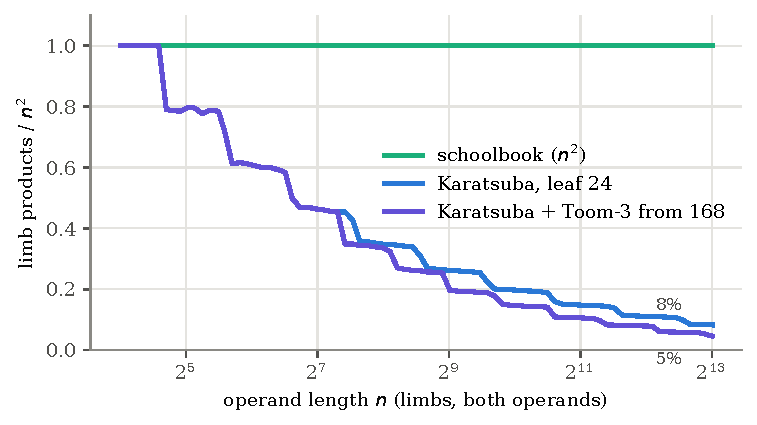
\includegraphics[width=0.8\textwidth]{figures/mul_counts.pdf}
\caption{Limb products needed, as a fraction of schoolbook's $n^2$, for the library's
recursion (leaf at 24 limbs, Toom-3 levels from 168 limbs). Computed exactly by
\file{figures/make\_figures.py}. Fewer products is not the whole story: the extra
additions and memory traffic are why the crossover sizes have to be measured.}
\label{fig:mulcounts}
\end{figure}

\subsection{Where the recursion stops}

Each Karatsuba level costs some additions, subtractions and bookkeeping. For short
pieces that overhead is larger than the multiplication it saves. The recursion therefore
stops at \code{BIGMATH\_KARATSUBA\_THRESHOLD} $= 24$ limbs and hands the piece to the
schoolbook kernel.

This cutoff has moved over time, which shows how measurement-driven it is: 48 limbs in
May 2026, 32 in June after the NTT got faster, and 24 in November after the flag-chain
kernels (\cref{sec:flagchain}) made Karatsuba's own additions cheaper. Cheaper overhead
means one more level of recursion pays off.

\subsection{Unequal sizes: slicing}

What if one number is much longer than the other, say $5000 \times 100$ limbs? Splitting
both ``in half'' makes no sense, because the short one has no high half. When one operand
is at least twice as long as the other, BigMath \emph{slices} the long operand into pieces
as long as the short one, multiplies each piece by the short operand (a balanced product),
and adds the pieces at their offsets.

\begin{figure}[ht]
\centering
\begin{tikzpicture}[x=1cm,y=1cm]
  \foreach \k in {0,...,4} {
    \fill[sBlue!18,draw=ink2] (\k*2.1,0) rectangle +(2,0.5);
    \node[font=\footnotesize] at (\k*2.1+1,0.25) {piece \k};
  }
  \node[lbl,anchor=east] at (-0.2,0.25) {long $x$};
  \fill[sOrange!25,draw=ink2] (0,-0.9) rectangle +(2,0.5);
  \node[font=\footnotesize] at (1,-0.65) {$y$};
  \node[lbl,anchor=east] at (-0.2,-0.65) {short $y$};
  \foreach \k in {0,...,4} {
    \draw[draw=ink2,fill=paper] (\k*2.1,-1.7-\k*0.45) rectangle +(4,0.38);
    \node[font=\tiny] at (\k*2.1+2,-1.51-\k*0.45) {piece \k\ $\times\ y$};
  }
  \node[lbl,anchor=west,align=left] at (11.3,-2.4) {each a balanced\\Karatsuba product,\\added at its offset};
\end{tikzpicture}
\caption{Slicing an unbalanced product into balanced ones.}
\end{figure}

The cost is the number of pieces times the cost of one balanced product: roughly
$n_{\max} \cdot K(n_{\min}) / n_{\min}$, where $K(m)$ is the cost of an $m \times m$
Karatsuba product. It grows \emph{linearly} with the long operand, at a rate set by the
short one. This is the key to choosing between Karatsuba and the NTT for lopsided shapes
(\cref{sec:arearule}).

\begin{pitfall}
Before slicing, the code just clamped the split point. For very lopsided shapes the
recursion then peeled off only a few limbs per level, ran $n_{\max}/n_{\min}$ levels deep
instead of $\log_2 n$, and its scratch space grew like $n_{\max}^2/n_{\min}$. On shapes the
dispatcher really sent there (for example $1214 \times 65$ limbs) that overflowed the
workspace buffer. Slicing fixed both the speed and the memory bound (about $4 n_{\max}$).
\end{pitfall}

\begin{perfnote}
The recursive multiplier reads operand ranges through pointers and partitions a
workspace sized before recursion starts. Requests of up to 2\,048 scratch limbs
use a stack buffer. Larger requests use heap storage. Inner calls write the
output and middle term directly. An earlier vector-based Karatsuba square lost
to plain multiplication at 128 limbs because of allocation and zero-fill costs.
\end{perfnote}

\section{Toom-3: split in three}
\label{sec:toom}

Karatsuba splits into halves. Why not thirds? Splitting into three parts gives
nine sub-products done naively; Toom-Cook (Andrei Toom 1963, Stephen Cook 1966) gets by
with \emph{five}. The cost becomes $n^{\log_3 5} \approx n^{1.465}$.

\subsection{The polynomial view}

Write each operand as a polynomial in the split point $X$:
\[
a = a_2 X^2 + a_1 X + a_0 \quad\longrightarrow\quad p(x) = a_2 x^2 + a_1 x + a_0 .
\]
Then $a \cdot b$ is the polynomial product $r(x) = p(x)\,q(x)$ evaluated at $x = X$. The
product has degree 4, so it has five unknown coefficients $r_0,\dots,r_4$. A degree-4
polynomial is fixed by its values at any five points. So:

\begin{enumerate}
  \item \textbf{Evaluate} $p$ and $q$ at five points. BigMath uses $0, 1, -1, 2$ and
        ``$\infty$'' (which simply means the top coefficient).
  \item \textbf{Multiply} the values pairwise: five products, each about one third as long
        as the inputs. These are done recursively.
  \item \textbf{Interpolate}: recover $r_0,\dots,r_4$ from the five values.
  \item \textbf{Recompose}: $a b = r_4 X^4 + r_3 X^3 + r_2 X^2 + r_1 X + r_0$, adding the
        overlapping pieces with carries.
\end{enumerate}

\begin{figure}[ht]
\centering
\begin{tikzpicture}[node distance=4mm and 9mm]
  \node[box,fill=sViolet!12] (in) {$a = (a_2, a_1, a_0)$\\$b = (b_2, b_1, b_0)$};
  \node[box,right=of in,fill=paper] (ev) {evaluate at\\$0,\ 1,\ -1,\ 2,\ \infty$};
  \node[box,right=of ev,fill=sViolet!12] (mul) {5 products\\of size $n/3$};
  \node[box,right=of mul,fill=paper] (int) {interpolate\\$r_0 \dots r_4$};
  \node[box,right=of int,fill=sViolet!12] (out) {$a \cdot b$};
  \draw[arr] (in) -- (ev); \draw[arr] (ev) -- (mul); \draw[arr] (mul) -- (int); \draw[arr] (int) -- (out);
  \node[lbl,below=1mm of mul] {(recursive)};
  \node[lbl,below=1mm of ev] {additions only};
  \node[lbl,below=1mm of int] {adds, shifts, $\div 2$, $\div 3$};
\end{tikzpicture}
\caption{Evaluate, multiply, interpolate. Only the middle step multiplies.}
\label{fig:evalinterp}
\end{figure}

\begin{example}[: $123 \times 456$ with Toom-3]
Split at $X = 10$: $p(x) = x^2 + 2x + 3$ and $q(x) = 4x^2 + 5x + 6$.

\textbf{Evaluate} (additions only):
\begin{center}
\begin{tabular}{lccccc}
\toprule
point & $0$ & $1$ & $-1$ & $2$ & $\infty$ \\
\midrule
$p$ & 3 & 6 & 2 & 11 & 1 \\
$q$ & 6 & 15 & 5 & 32 & 4 \\
\midrule
product $v$ & $v_0 = 18$ & $v_1 = 90$ & $v_{-1} = 10$ & $v_2 = 352$ & $v_\infty = 4$ \\
\bottomrule
\end{tabular}
\end{center}

\textbf{Interpolate} with Bodrato's sequence, the one the library uses. Every line is an
addition, a subtraction, or an exact division by 2 or 3:
\begin{align*}
v_2 &\leftarrow (v_2 - v_{-1})/3 = (352 - 10)/3 = 114 && = r_1 + r_2 + 3r_3 + 5r_4\\
v_{-1} &\leftarrow (v_1 - v_{-1})/2 = (90 - 10)/2 = 40 && = r_1 + r_3\\
v_1 &\leftarrow v_1 - v_0 = 90 - 18 = 72 && = r_1 + r_2 + r_3 + r_4\\
v_2 &\leftarrow (v_2 - v_1)/2 = (114 - 72)/2 = 21 && = r_3 + 2 r_4\\
v_1 &\leftarrow v_1 - v_{-1} - v_\infty = 72 - 40 - 4 = 28 && = r_2\\
v_2 &\leftarrow v_2 - 2 v_\infty = 21 - 8 = 13 && = r_3\\
v_{-1} &\leftarrow v_{-1} - v_2 = 40 - 13 = 27 && = r_1
\end{align*}
So $r = (r_4, r_3, r_2, r_1, r_0) = (4, 13, 28, 27, 18)$.

\textbf{Recompose} at $x = 10$: $40000 + 13000 + 2800 + 270 + 18 = 56088$, and
$123 \times 456 = 56088$. Five small products replaced nine.
\end{example}

\begin{another}[: Karatsuba is Toom-2]
The product $(a_1x + a_0)(b_1x + b_0)$ has degree 2. At $0$, $1$ and $\infty$ it
gives Karatsuba's three products $a_0b_0$, $(a_0 + a_1)(b_0 + b_1)$ and $a_1b_1$.
Subtracting $z_0$ and $z_2$ gives the middle coefficient. Toom-$k$ uses $2k-1$
points. More pieces lower the exponent and raise evaluation and interpolation
costs. \Cref{ch:ntt} takes the same idea further.
\end{another}

\subsection{Why the sequence runs on unsigned numbers}

Look at the right-hand column of the interpolation: every intermediate value is a
combination of the $r_i$ with non-negative weights, and the $r_i$ themselves are never
negative (they are sums of products of limbs). So no intermediate value is ever negative,
and the whole interpolation runs on plain unsigned limb arrays with the fast kernels. Only
$v_{-1}$ can be negative, since $p(-1)$ and $q(-1)$ can be; its sign is tracked separately
and folded into the first two steps. The exact division by 3 is a multiplication by the
inverse of 3 modulo $2^{64}$ (\code{0xAAAA\ldots AAB}), which is much cheaper than a real
division.

\subsection{Where Toom-3 is used}

Toom-3 lives \emph{inside} the Karatsuba recursion: at each level, if the shorter operand
has at least \code{BIGMATH\_MUL\_TOOM33\_THRESHOLD} $= 168$ limbs (160 for squares) and both
operands have a non-empty top third, the level splits three ways; otherwise it halves as
usual. Because the choice is made at every level, every sub-product picks the best split
for its own size, including the pieces of sliced unbalanced products and the products
inside division.

Measured on balanced products (microseconds):

\begin{center}
\begin{tabular}{lrrrrrrr}
\toprule
limbs & 160 & 176 & 192 & 224 & 384 & 512 & 768 \\
\midrule
Karatsuba only & 7.38 & 9.20 & 10.21 & 13.40 & 31.60 & 48.76 & 96.44 \\
with Toom-3 & 7.37 & 8.60 & 9.55 & 12.64 & 28.76 & 45.73 & 86.53 \\
\bottomrule
\end{tabular}
\end{center}

A 5--10\% gain. Modest, because balanced products from about 310 limbs go to the NTT when
the thread pool is awake. Toom-3 matters most for cold calls and for the unbalanced pieces
and division sub-products that stay below the NTT.

\begin{practice}
The public multiplication operator reaches the limb-based Toom-3 through
Karatsuba. The optional four-way split has a default cutoff of $10^6$ limbs,
effectively out of reach before the NTT takes over.
\end{practice}

\clearpage
\section{Toom-5: nine products from five pieces}
\label{sec:toomfive}

Take five chunks from each operand, keeping them in order from low to high.
Divide the longer length by five and round up to get the chunk width $k$
in limbs. Missing high chunks are zero. Each chunk's place value is a
power of $X=B^k$.
For example, the first operand is $a_0+a_1X+\cdots+a_4X^4$. Think of
that expression as a recipe. Replace $X$ temporarily by a small number
$x$ and you can mix the five chunks using additions and short integer
multiplications. Mix both inputs with the same $x$, then multiply the
two mixed values.

\begin{figure}[H]
\centering
\begin{tikzpicture}[x=1.26cm,y=0.59cm]
  \foreach \i in {0,...,4} {
    \node[lbl] at (\i,0.83) {$b_{\i}$};
    \node[lbl] at (-0.9,-\i) {$a_{\i}$};
    \foreach \j in {0,...,4} {
      \pgfmathtruncatemacro{\degree}{\i+\j}
      \ifnum\degree=4
        \node[box,minimum width=11mm,fill=sViolet!25] at (\j,-\i) {$a_{\i}b_{\j}$};
      \else
        \node[box,minimum width=11mm,fill=paper] at (\j,-\i) {$a_{\i}b_{\j}$};
      \fi
    }
  }
  \node[box,fill=sViolet!15,text width=40mm] (middle) at (7.15,-2)
    {\textbf{One output coefficient}\\[1pt]$c_4$ adds the five\\highlighted products};
  \draw[arr] (4.46,0) -- (5.03,0) |- (middle.west);
\end{tikzpicture}
\caption{Direct multiplication makes 25 chunk products. All entries with
$i+j=4$ contribute to the same power of the chunk base. The whole grid gives
nine coefficients, $c_0$ through $c_8$.}
\end{figure}

Toom-5 recovers those same nine coefficients from nine products of mixed
values. Two come straight from the ends. The low chunks give $c_0$ and
the high chunks give $c_8$, written as the values at $0$ and $\infty$.
Seven other points each supply one equation in the seven middle
coefficients. Solving those equations is called \emph{interpolation}.
The hand example uses integer points. The limb implementation uses
$\pm1/2,\pm1,\pm2$ and $4$, so it can scale the evaluations by powers of two.

\begin{figure}[H]
\centering
\begin{tikzpicture}[node distance=5mm]
  \node[box,fill=sViolet!12] (input) {5 chunks\\per operand};
  \node[box,right=of input] (mix) {mix at the same\\9 points};
  \node[box,fill=sViolet!12,right=of mix] (mul) {9 smaller\\products};
  \node[box,right=of mul] (solve) {recover the\\9 coefficients};
  \node[box,fill=sViolet!12,right=of solve] (out) {shift, add,\\and carry};
  \draw[arr] (input) -- (mix);
  \draw[arr] (mix) -- (mul);
  \draw[arr] (mul) -- (solve);
  \draw[arr] (solve) -- (out);
\end{tikzpicture}
\caption{Each mixed product replaces work on the original chunks. Interpolation
puts the products back into their original place values.}
\end{figure}

Ideally a five-way recursion grows like $n^{\log_5 9}\approx n^{1.365}$,
versus $n^{\log_3 5}\approx n^{1.465}$ for Toom-3. Evaluation and
interpolation involve many extra passes over the pieces, which matter
at the sizes where the two methods compete.

\newpage
\subsection{Worked example with five decimal chunks}

Multiply $12345$ by $12121$ using one decimal digit per chunk, so $X=10$.
At $x=1$ each mixed value is just the sum of its digits. At $x=-1$ the
second input gives $1-2+1-2+1=-1$. The sign travels with the product.
The final column uses the two high digits.

\begin{center}
\small
\begin{tabular}{lrrrrrrrrr}
\toprule
point $x$ & $0$ & $1$ & $-1$ & $2$ & $-2$ & $3$ & $-3$ & $4$ & $\infty$ \\
\midrule
first input & 5 & 15 & 3 & 57 & 9 & 179 & 47 & 453 & 1 \\
second input & 1 & 7 & $-1$ & 41 & 1 & 151 & 31 & 409 & 1 \\
product $r(x)$ & 5 & 105 & $-3$ & 2337 & 9 & 27029 & 1457 & 185277 & 1 \\
\bottomrule
\end{tabular}
\end{center}

The endpoints give $c_0=5$ and $c_8=1$. Subtract their contributions to get
$h(x)=r(x)-5-x^8$. At $x$ and $-x$ the even powers have the same sign and
the odd powers have opposite signs. Half the sum isolates the even part,
and half the difference isolates the odd part. At $x=1$ these are
$(99-9)/2=45$ and $(99+9)/2=54$. Dividing the even part by $x^2$ and the
odd part by $x$ leaves two short polynomials in $t=x^2$.

\begin{center}
\small
\begin{tabular}{lrrrr}
\toprule
$t=x^2$ & 1 & 4 & 9 & 16 \\
\midrule
$E(t)=c_2+c_4t+c_6t^2$ & 45 & 228 & 853 & $2400$ \\
$O(t)=c_1+c_3t+c_5t^2+c_7t^3$ & 54 & 582 & 4262 & $20334$ \\
\bottomrule
\end{tabular}
\end{center}

Here is one way to solve the equations by hand. The first two slopes of
$E$ are $(228-45)/3=61$ and $(853-228)/5=125$. Their difference divided
by $9-1$ is $8$. Thus
$E(t)=45+61(t-1)+8(t-1)(t-4)=16+21t+8t^2$. This gives $E(16)=2400$.
The extra reading at $x=4$ gives $O(16)=(119736-16\cdot2400)/4=20334$.
Applying the same slope calculation to $O$ gives
\[
O(t)=54+176(t-1)+70(t-1)(t-4)+4(t-1)(t-4)(t-9)
    =14+22t+14t^2+4t^3 .
\]
The limb implementation uses the same slope calculation. It scales its
fractional samples by powers of two so the grid and the polynomial
coefficients are integers. Each division in interpolation is exact.

\begin{center}
\small
\begin{tabular}{lrrrrrrrrr}
\toprule
place, low to high & 0 & 1 & 2 & 3 & 4 & 5 & 6 & 7 & 8 \\
\midrule
raw coefficient & 5 & 14 & 16 & 22 & 21 & 14 & 8 & 4 & 1 \\
carry in & 0 & 0 & 1 & 1 & 2 & 2 & 1 & 0 & 0 \\
digit after carry & 5 & 4 & 7 & 3 & 3 & 6 & 9 & 4 & 1 \\
\bottomrule
\end{tabular}
\end{center}

At place 2, $16+1=17$ writes $7$ and sends a carry of $1$. Read the final
digits from high to low to get $149\,633\,745$.

\begin{practice}
\file{Toom5Multiplication.h} provides a direct call to the limb-based
implementation. It uses Karatsuba below 512 limbs in the longer operand
and for the legacy radix. The automatic dispatcher uses the existing
recursive and NTT paths. See \file{BENCHMARK.md} for the higher Toom sweep.
\end{practice}

\newpage
\section{Toom-6.5 and Toom-8.5: unequal splits}
\label{sec:toomhalf}

In the half-step variants, one operand gets an extra chunk slot. Toom-6.5
uses seven slots for the longer operand and six for the shorter.
Toom-8.5 uses nine and eight. Both operands use the same chunk width.
When the extra high slot lies beyond the end of an operand, it contributes
zero. For example, a $700\times600$-limb Toom-6.5 product uses 100 limbs
per slot. Each input fits its row exactly.

\begin{figure}[H]
\centering
\begin{tikzpicture}[x=0.96cm,y=0.64cm]
  \node[lbl,anchor=east] at (-0.51,0) {Toom-6.5};
  \node[lbl,anchor=east] at (-0.51,-2.35) {Toom-8.5};
  \foreach \i in {0,...,8} {
    \ifnum\i<7
      \node[box,fill=sViolet!16,minimum width=8mm] at (\i,0.45) {\footnotesize $a_{\i}$};
    \fi
    \ifnum\i<6
      \node[box,fill=sAqua!16,minimum width=8mm] at (\i,-0.45) {\footnotesize $b_{\i}$};
    \fi
    \node[box,fill=sViolet!16,minimum width=8mm] at (\i,-1.9) {\footnotesize $a_{\i}$};
    \ifnum\i<8
      \node[box,fill=sAqua!16,minimum width=8mm] at (\i,-2.8) {\footnotesize $b_{\i}$};
    \fi
  }
  \node[lbl,anchor=west] at (6.65,0) {12 pointwise products};
  \node[lbl,anchor=west] at (8.65,-2.35) {16 pointwise products};
\end{tikzpicture}
\caption{The extra slot makes the product degree odd. Two products come
from the ends of the input rows. The remaining products come in pairs
evaluated at a positive point and its negative.}
\end{figure}

For seven by six slots, the two input recipes have degrees six and five,
so their product has degree eleven. Twelve readings determine its
coefficients. Two are the endpoints. The other ten come from
$\pm1/4,\pm1/2,\pm1,\pm2,\pm4$. Adding paired results isolates the even
powers and subtracting them isolates the odd powers. After removing the
endpoints, five even and five odd coefficients are left.

With nine by eight slots the degrees are eight and seven, so there are
sixteen readings. The extra pairs are $\pm1/8$ and $\pm8$. Squaring the
positive points gives a grid whose neighboring values differ by a factor
of four. The code scales it to $1,4,16,\ldots$ and uses the divided
differences from the Toom-5 example to recover the coefficients. Shifts
handle the powers of two. Multiplication by an inverse modulo the limb
base handles each remaining odd divisor exactly.

BigMath's two half-step kernels share the buffer and interpolation code
with limb-based Toom-5. Each forces one outer split, then uses the existing
Karatsuba and Toom-3 recursion for its smaller products. The design uses
the paired powers-of-two idea described in the
\href{https://gmplib.org/manual/Higher-degree-Toom_0027n_0027half}{GNU MP manual}.
